% Project report for CS787. Build:  cd paper && python build_assets.py && tectonic main.tex
\documentclass[12pt,a4paper]{report}

% ---------------------------------------------------------------- fill these in
\newcommand{\reporttitle}{Wrong Names in Natural Language Autoencoder Explanations}
\newcommand{\studentname}{Tanvi Pooranmal Meena}
\newcommand{\rollno}{231085}
\newcommand{\programme}{Department of Mechanical Engineering}
\newcommand{\instructor}{Prof.\ Arnab Bhattacharya}
\newcommand{\course}{CS787: Generative Artificial Intelligence}
\newcommand{\department}{Department of Computer Science and Engineering}
\newcommand{\institute}{Indian Institute of Technology Kanpur}
\newcommand{\semester}{2026--27, Semester I}
\newcommand{\reportdate}{November 2026}
% ----------------------------------------------------------------

\usepackage[T1]{fontenc}
\usepackage{lmodern}
\usepackage[margin=1in]{geometry}
\usepackage{microtype}
\usepackage{amsmath,amssymb}
\usepackage{graphicx}
\usepackage{booktabs}
\usepackage{array}
\usepackage{xcolor}
\usepackage{enumitem}
\usepackage[font=small,labelfont=bf]{caption}
\usepackage{setspace}
\usepackage{titlesec}
\usepackage{aurical}
\usepackage{tikz}
\usetikzlibrary{arrows.meta,positioning}
\usepackage[numbers,sort&compress]{natbib}
\usepackage[colorlinks=true,linkcolor=black,citecolor=black,urlcolor=blue!50!black]{hyperref}

\setstretch{1.15}
\titleformat{\chapter}[hang]{\LARGE\bfseries}{\thechapter}{0.8em}{}
\titleformat{name=\chapter,numberless}[hang]{\LARGE\bfseries}{}{0pt}{}
\titlespacing*{\chapter}{0pt}{-12pt}{16pt}
\setlist{itemsep=2pt,topsep=4pt}
\graphicspath{{figs/}}
% keep floats with their text instead of on pages of their own
\renewcommand{\topfraction}{0.9}\renewcommand{\bottomfraction}{0.8}\renewcommand{\textfraction}{0.08}
\renewcommand{\floatpagefraction}{0.85}\setcounter{topnumber}{3}\setcounter{totalnumber}{4}

% a passage or explanation quoted from the data
\newenvironment{sample}[1]{\par\smallskip\noindent\begin{minipage}{\linewidth}\small\textbf{#1}\par\vspace{2pt}%
  \begin{quote}\itshape}{\end{quote}\end{minipage}\par\smallskip}
\newcommand{\true}[1]{\textbf{#1}}
\newcommand{\wrong}[1]{\textbf{\underline{#1}}}

\begin{document}

\pagenumbering{roman}
\begin{titlepage}
\centering
\vspace*{1.5cm}
{\huge\bfseries \reporttitle\par}
\vspace{2.2cm}
{\large A project report submitted for the course\par}
\vspace{0.3cm}
{\large\bfseries \course\par}
\vspace{2.2cm}
{\large by\par}
\vspace{0.3cm}
{\Large\bfseries \studentname\par}
\vspace{0.2cm}
{\large Roll No.\ \rollno\par}
\vspace{0.2cm}
{\large \programme\par}
\vspace{1.6cm}
{\large Course instructor\par}
\vspace{0.3cm}
{\Large \instructor\par}
\vfill
{\large \department\par}
\vspace{0.2cm}
{\large\bfseries \institute\par}
\vspace{0.4cm}
{\large \reportdate\par}
\end{titlepage}

\chapter*{Certificate}
\addcontentsline{toc}{chapter}{Certificate}

This is to certify that the project report titled \emph{``\reporttitle: Where Natural Language Autoencoders
Lose Specifics, and What Brings Them Back''}, submitted by \textbf{\studentname} (Roll No.\ \rollno) for the
course \course, is a record of work carried out by the student under my guidance during the academic year
\semester.

\vspace{3cm}

\noindent
\begin{minipage}[t]{0.45\linewidth}
Date: \rule{4cm}{0.4pt}\\[0.4cm]
Place: Kanpur
\end{minipage}\hfill
\begin{minipage}[t]{0.5\linewidth}
\raggedleft
\rule{6.5cm}{0.4pt}\\[0.2cm]
\instructor\\
\department\\
\institute
\end{minipage}

\chapter*{Declaration}
\addcontentsline{toc}{chapter}{Declaration}

I declare that this report describes my own work, carried out for the course \course. Where I have used the
ideas, models, data or code of others, I have cited the source. The report has not been submitted, in whole or
in part, for any other course or degree.

I used an AI coding assistant to help write and run the code and analysis scripts. I chose the questions, directed the experiments, checked the results, and I take responsibility for
everything reported here.

\vspace{2.2cm}

\noindent
\begin{minipage}[t]{0.45\linewidth}
Date: 13 November 2026\\[0.4cm]
Place: Kanpur
\end{minipage}\hfill
\begin{minipage}[t]{0.5\linewidth}
\raggedleft
\makebox[6.5cm][c]{
\includegraphics[height=1.25cm]{signature}}\\[-0.25cm]
\rule{6.5cm}{0.4pt}\\[0.2cm]
\studentname\\
Roll No.\ \rollno\\
\programme
\end{minipage}

\chapter*{Acknowledgements}
\addcontentsline{toc}{chapter}{Acknowledgements}

I thank \instructor\ for the course, and for two pieces of advice this report tries to follow: that a
narrow question answered carefully is worth more than a broad one answered loosely, and that understanding
why something behaves the way it does matters more than making it work.

This project would not exist without the authors of the Natural Language Autoencoders work, who released
their trained models, their training code and unusually candid documentation. Everything here is built on
their Qwen2.5-7B checkpoints.

The experiments ran on a laptop, on free Kaggle GPUs and on rented RunPod GPUs. The passages come from
Wikipedia, and the name lists from GeoNames, WordNet and spaCy.

\chapter*{Abstract}
\addcontentsline{toc}{chapter}{Abstract}

A natural language autoencoder (NLA) explains an activation inside a language model by writing a paragraph
about it, and is trained so that a second model can rebuild the activation from the paragraph. The
explanations read well, but they sometimes name the wrong specific: a city, person or instrument that was
never in the text. This report measures that failure on the released NLA for Qwen2.5-7B, using 6{,}000
Wikipedia passages about 60 entities, and asks how often it happens, why, and what removes it.

Four findings come out. First, specifics fade from the explanation faster than from the activation: sixteen
tokens after an entity, the explanation names it 7.5\% of the time while a linear probe still reads it 35\%
of the time, and 22\% of explanations contain a wrong name of the same type. Second, the training objective
barely notices: editing a wrong name out changes the reconstruction cosine by about 0.002. Third, agreement
between sampled explanations separates true names from wrong ones; keeping only names that two of four
samples share removes 74\% of wrong names and keeps 77\% of true ones, with no training, and most of that
signal is already present in one explanation's token probabilities. Fourth, the explanation survives
intervention: fine-tuning on reconstruction alone changes nothing, a cost on unsupported names cuts wrong
names by 8\% on held-out passages, and rewarding the true name does not bring it back.

The practical advice is simple: trust the gist of an NLA explanation, and do not trust a name unless
several samples agree on it.

\tableofcontents
\listoffigures
\listoftables
\clearpage
\pagenumbering{arabic}

\chapter{Introduction}
\label{ch:intro}

\section{Motivation}

A natural language autoencoder (NLA) takes one activation vector from inside a language model and writes a
short paragraph describing what that vector contains~\cite{frasertaliente2026nla}. A second model reads the
paragraph and tries to rebuild the vector. If the rebuilt vector is close to the original, the paragraph must
have carried most of the information, so it can be read as an explanation of the activation. The appeal is
obvious: instead of a list of feature numbers, you get English.

The trouble is that English is persuasive. Here is a passage from Wikipedia, and what the released NLA for
Qwen2.5-7B wrote about the activation one token after the word \emph{cello}:

\begin{sample}{Passage (the model has read up to ``son'')}
\ldots It has since performed at the Wigmore Hall in London, and in many countries worldwide. A recording of
the \true{cello} son$|$atas of Antonio Vivaldi \ldots
\end{sample}

\begin{sample}{Explanation written by the NLA}
Biographical music description format with British classical composer context \ldots\ Final token ``son'' is
a truncated word mid-expression (``the \wrong{piano} son''), part of a noun phrase listing the completed
work's content (``the \wrong{piano} sonatas''), strongly expecting ``atas'' \ldots
\end{sample}

Most of this is right. The explanation knows the text is about classical music in a British setting, it
knows the current word is the first half of ``sonatas'', and it knows which letters come next.
The one thing it gets wrong is the specific: the instrument was a cello, and the explanation says piano, twice,
with no hint of doubt. A reader who trusts the explanation walks away believing the model was thinking about a
piano.

This report is about that failure. I call the cello a \emph{specific}: a named entity that is really in the
text. The gist (classical music, a recording, sonatas) survives the round trip through language. The
specific often does not, and what replaces it is a confident wrong name of the same kind.

\section{Prior Work}

Wrong specifics in NLA explanations are a known problem, and several groups have worked on it.

\begin{itemize}
\item \emph{The NLA authors} report it themselves~\cite{frasertaliente2026nla}: explanations are usually right
about the theme and can be wrong about the detail, and a claim that recurs across neighbouring tokens is more
likely to be true.
\item \emph{Audits.} Dingeto~\cite{dingeto2026recap} finds that on the released Qwen2.5-7B verbalizer only
about 2\% of specific claims are ones the reconstruction depends on. Denamgana\"i~\cite{denamganai2026monitorability}
finds that a true account beats a rival differing in one claim only 60\% of the time.
\item \emph{Fixes by retraining.} Flow-NLA~\cite{lek2026flownla} replaces point reconstruction with a model of
all the activations an explanation is compatible with. Hong et al.~\cite{hong2026grounding} add a grounding
reward for names, numbers and quotations. Dingeto's RECAP~\cite{dingeto2026recap} trains the target model
itself so that chosen content stays readable.
\item \emph{Neighbouring tools.} Other ways of turning activations into text include the logit
lens~\cite{nostalgebraist2020logitlens}, Patchscopes~\cite{ghandeharioun2024patchscopes} and
SelfIE~\cite{chen2024selfie}; sparse autoencoders are the main
alternative~\cite{bricken2023monosemanticity,cunningham2023sparse}. Linear probes~\cite{alain2016probes} test
what an activation holds, and agreement between samples is a standard signal for invented content in
ordinary generation~\cite{manakul2023selfcheckgpt,wang2023selfconsistency}.
\end{itemize}

\section{Question}

I ask one narrow question and try to answer it carefully:

\begin{quote}
When an NLA explanation names an entity, how often is the name wrong, why does that happen, and what removes
the wrong names?
\end{quote}

The middle part matters most. The aim is to understand why the verbalizer behaves this way, not to ship a
better one. So \emph{how often} is a measurement against a baseline, \emph{why} is tested with an
intervention, and the fixes are there mainly as checks on the explanation: if wrong names are free under the
training objective, more training on that objective should not remove them, and a penalty on them should.

\section{Contributions}

Working with the released Qwen2.5-7B NLA and 6{,}000 Wikipedia passages about 60 entities, this report adds
four things to the work above. As far as I know each is new. None of them retrains an NLA from scratch or
needs the source text at inference.

\begin{enumerate}
\item \textbf{A fade curve with a ceiling.} Names are tracked token by token after the entity, next to a probe
on the same activations, which separates what the verbalizer drops from what the model no longer holds.
Sixteen tokens after the entity the explanation names it 7.5\% of the time while the probe still reads it
35\% of the time, and between a fifth and a half of all explanations contain a wrong name of the same type
(Chapter~\ref{ch:fading}).

\item \textbf{A price for each kind of name.} Sharpening Dingeto's 2\% finding, an edit test prices wrong and
true names separately. A wrong name is worth about 0.002 of reconstruction score. The true name is worth
0.21 at the entity's token and 0.016 one token later (Chapter~\ref{ch:incentives}).

\item \textbf{Agreement as a filter, and where it comes from.} The NLA authors' observation about neighbouring
tokens is applied to repeated samples of one activation and measured. A name in one of four samples is right
6\% of the time; a name in all four, 64\%. Keeping names that two samples agree on removes 74\% of the wrong
names and keeps 77\% of the true ones, with no training and no labels. Most of this signal is token-level
confidence that a single explanation already carries (Chapter~\ref{ch:agreement}).

\item \textbf{Rewards as tests.} Small fine-tunes of the released verbalizer check the incentive account. More
reconstruction leaves wrong names untouched. A cost on names the other samples do not support cuts them by
5 to 8\% on held-out passages, in two independent runs, without losing true names. Rewarding the true name
does not bring it back (Chapter~\ref{ch:finetuning}).
\end{enumerate}

Along the way I found that the usage example published with the models reads activations one layer too early,
which silently lowers reconstruction quality; Appendix~\ref{app:layer} documents the bug and the check that confirmed the
fix. Every table in this report is
generated from saved outputs by one command.

\paragraph{Availability.} Everything needed to check or rerun the work is in three places:
{\small
\begin{itemize}
\item Code, explanations and result tables:\\ \url{https://github.com/tanvincible/nla-wrong-names}
\item Fine-tuned adapters:\\ \url{https://huggingface.co/tanvincible/nla-qwen2.5-7b-L20-av-specifics-lora}
\item Activations, caches and training samples:\\ \url{https://huggingface.co/datasets/tanvincible/nla-specifics-artifacts}
\end{itemize}}

\chapter{Background}
\label{ch:background}

\section{Autoencoders}

An autoencoder is a pair of functions trained together: an encoder that squeezes an input into a smaller
code, and a decoder that rebuilds the input from the code~\cite{hinton2006reducing}. Nothing tells the
encoder what the code should mean. The only pressure is that the decoder has to succeed, so the code ends up
holding whatever the decoder needs most.

That last sentence is the key to this whole report. An autoencoder keeps what helps reconstruction and is
indifferent to everything else. If two different inputs can be rebuilt almost equally well from the same
code, the encoder has no reason to tell them apart.

\section{NLA Design}

A natural language autoencoder~\cite{frasertaliente2026nla} is an autoencoder whose input is an activation
vector from a language model and whose code is a paragraph of English. Figure~\ref{fig:nla} shows the three
models involved.

\begin{figure}[t]
\centering
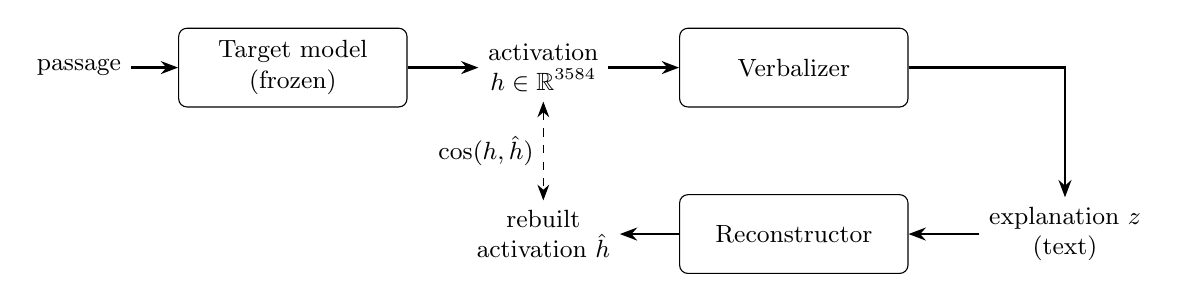
\begin{tikzpicture}[
  box/.style={draw, rounded corners=3pt, minimum height=1.0cm, minimum width=2.9cm, align=center, font=\small},
  data/.style={align=center, font=\small},
  arr/.style={-{Stealth[length=2.2mm]}, thick}]
\node[box] (target) {Target model\\(frozen)};
\node[data, left=0.6cm of target] (text) {passage};
\node[data, right=0.9cm of target] (h) {activation\\$h \in \mathbb{R}^{3584}$};
\node[box, right=0.9cm of h] (av) {Verbalizer};
\node[box, below=1.1cm of av] (ar) {Reconstructor};
\node[data, right=0.9cm of ar] (z) {explanation $z$\\(text)};
\node[data] (hh) at (h |- ar) {rebuilt\\activation $\hat h$};
\draw[arr] (text) -- (target);
\draw[arr] (target) -- (h);
\draw[arr] (h) -- (av);
\draw[arr] (av.east) -| (z.north);
\draw[arr] (z) -- (ar);
\draw[arr] (ar) -- (hh);
\draw[{Stealth[length=2mm]}-{Stealth[length=2mm]}, dashed] (h) -- node[left, font=\small]{$\cos(h,\hat h)$} (hh);
\end{tikzpicture}
\caption[The three models in a natural language autoencoder]{The three models in a natural language
autoencoder. The target model reads a passage; one activation $h$ is taken from its residual stream. The
verbalizer turns $h$ into text, and the reconstructor turns the text back into a vector. Training rewards a
high cosine between $h$ and $\hat h$.}
\label{fig:nla}
\end{figure}

\begin{description}
\item[Target model.] The model being explained. Here it is Qwen2.5-7B-Instruct~\cite{qwen25}, and the
activation is the residual stream after block 20 of 28, a vector of 3{,}584 numbers at one token position.
\item[Verbalizer.] A copy of the target model, fine-tuned to describe an activation. The vector is rescaled
and placed into a fixed prompt as if it were the embedding of a single token; the verbalizer then writes an
explanation, one token at a time. This is the encoder.
\item[Reconstructor.] Another fine-tuned copy, cut off after the extraction layer, with a linear layer on
top. It reads the explanation and outputs a vector. This is the decoder.
\end{description}

Both vectors are scaled to unit length before they are compared, so the reconstruction error is
$2(1-\cos(h,\hat h))$: only the direction matters. I report the cosine throughout.

The authors train in three stages. The reconstructor first learns to predict activations from text. The
verbalizer first learns to imitate explanations that a large language model, called through an API, wrote
for each position. Then the two are trained together: the verbalizer by reinforcement learning
(GRPO~\cite{shao2024deepseekmath}), with the reconstruction score as its reward, and the reconstructor by
ordinary regression on whatever the verbalizer writes. In this last stage the only reward is reconstruction.

The explanations the released verbalizer writes have a steady three-part shape, visible in the example in
Chapter~\ref{ch:intro}. The first paragraph gives the genre and topic of the text. The second quotes or
paraphrases the sentence being read. The third describes the final token and lists what is expected next. I
use this shape later, to ask whether wrong names sit in the part that describes the context or the part that
predicts the continuation.

\section{Specifics}

By a \emph{specific} I mean a named entity that appears in the passage the target model read: a particular
country, city, person, animal, food or instrument. An explanation can do three things with it.

\begin{itemize}
\item Name it. I call this a \emph{true name}.
\item Name a different entity of the same type that is not in the passage, as with the piano above. I call
this a \emph{wrong name}.
\item Name nothing of that type, and describe the passage only in general terms.
\end{itemize}

The third option is not a failure. If the activation no longer holds the entity, the faithful thing to say
is nothing. The failure this report studies is the second one, because a wrong name is indistinguishable from
a true one to anyone reading the explanation without the passage in front of them.

Specifics are the natural place to look for trouble. The gist of a passage (music, a biography, a list of
recordings) is shared by thousands of training examples and moves the activation a long way, so the
reconstructor depends on it and the verbalizer learns to report it. Which instrument it was moves the
activation much less. Chapter~\ref{ch:incentives} measures exactly how much less.

\chapter{Setup}
\label{ch:setup}

Everything in this report runs on the released NLA for Qwen2.5-7B-Instruct at layer~20. The target model,
the verbalizer and the reconstructor are used exactly as published, except in the fine-tuning experiments,
where a small adapter is added to the verbalizer. This chapter describes the data and the three measuring
instruments: a detector for names, a probe that says what the activation still holds, and the statistics.

\section{Data}

I chose 60 entities, ten of each of six types (Table~\ref{tab:entities}). Three types are proper nouns and
three are common nouns, so that the results do not depend on capital letters or on how well a named-entity
recogniser works.

\begin{table}[t]
\centering
\small
\begin{tabular}{@{}lp{0.78\linewidth}@{}}
\toprule
Type & Entities \\
\midrule
Country & France, Japan, Egypt, Brazil, Canada, India, Germany, Italy, Mexico, Russia \\
City & Paris, Tokyo, Cairo, Chicago, London, Berlin, Moscow, Sydney, Toronto, Rome \\
Person & Shakespeare, Napoleon, Einstein, Mozart, Darwin, Lincoln, Churchill, Gandhi, Picasso, Beethoven \\
Animal & dog, cat, horse, lion, tiger, elephant, wolf, eagle, rabbit, dolphin \\
Food & bread, cheese, rice, pasta, chocolate, pizza, butter, honey, potato, sugar \\
Instrument & piano, guitar, violin, cello, flute, trumpet, saxophone, clarinet, harp, banjo \\
\bottomrule
\end{tabular}
\caption{The 60 entities.}
\label{tab:entities}
\end{table}

For each entity I collected 100 passages from the November 2023 English Wikipedia dump, 6{,}000 in all. A
passage qualifies if the entity appears in it exactly once, none of the other nine entities of its type
appears, at least 50 tokens come before the entity, and 16 tokens come after it. Articles whose title
contains the entity are skipped, so that the passage is about something else and merely mentions the entity,
and each article contributes at most one passage per entity.

The passages are split per entity: 30 for testing, and of the remaining 70, 14 for validation and 56 for
fitting. That gives 1{,}800 test, 840 validation and 3{,}360 fitting passages. Test passages are never used
to fit a probe or to fine-tune anything.

\section{Activations}

For every passage I ran the target model and saved the layer-20 activation at six positions: the entity's
last token, and 1, 2, 4, 8 and 16 tokens after it. I call these \emph{distances}. Distance~0 is where the
model has just read the entity; distance~16 is roughly a sentence later.

Before trusting any number, I checked that my pipeline reproduces known reconstruction quality. I had an
earlier pilot run of the released models, written separately and run on different hardware, which gave a
mean cosine of 0.907 between original and rebuilt activations. Repeating that run's recipe, the pipeline
used here gives 0.908, and explains 75.0\% of the variance, in line with the roughly 75\% the authors report
for this model. Getting there required fixing an off-by-one in which layer is read, described in
Appendix~B. On Wikipedia passages the mean cosine is 0.893, a little lower.

\section{Explanations}

Generating explanations is the expensive step, so the main measurements use a fixed subset of the test set:
nine test passages per entity, chosen by a seeded shuffle before any explanation was generated, at distances
0, 1, 4 and 16. That is 540 passages and 2{,}160 activations. For each activation the verbalizer wrote four
explanations, sampled independently at temperature~1, for 8{,}640 explanations in total. Four samples per
activation is what later makes it possible to ask whether the samples agree.

\section{Name Detector}

Every result depends on deciding, for an explanation and its passage, which names are true and which are
wrong. The rules are:

\begin{itemize}
\item The explanation \textbf{names the true entity} if the entity, or one of a small fixed set of variants
(\emph{wolves} for wolf, \emph{puppy} for dog), appears as a whole word.
\item A \textbf{wrong name} is any other entity of the same type that appears in the explanation and does
\emph{not} appear in the passage. A same-type name that is in the passage is real content the explanation
got right, so it is not counted against it.
\end{itemize}

``Any other entity of the same type'' has to reach well beyond my ten. For countries I use every country in
GeoNames, for cities every city above 300{,}000 people, for people the spans a named-entity recogniser tags
as persons (spaCy's small English model~\cite{spacy}), and for animals, foods and instruments the
corresponding branches of WordNet~\cite{miller1995wordnet}, keeping a word only where that sense is its most
common one. The broad lists matter: about four in five of the wrong names found later are outside my list of
60 (Section~\ref{sec:wrongnames}).

The detector is imperfect, and I would rather say how than hide it. A hand check of 30 flagged explanations
found four kinds of false alarm: category words (\emph{bird}, \emph{mammal}), meals (\emph{dinner}), words
for people in general (\emph{humans}), and ``persons'' that were not proper nouns. The detector used
throughout drops these. What remains is that the recogniser sometimes misses or invents a person, ambiguous
words such as \emph{bear} and \emph{bass} are never detected, and adjectives such as \emph{French} never
count as a country. These errors affect every condition I compare in the same way, since the same detector
scores all of them, but they do mean the absolute rates carry more uncertainty than their intervals show.

\section{Probe Baseline}

A falling true-name rate could mean two things: the verbalizer is failing to report something the activation
holds, or the activation no longer holds it. To tell these apart I need an independent estimate of what the
activation holds.

I use a linear probe~\cite{alain2016probes}. For each type $t$ and distance $\delta$, a ten-way logistic
regression on the standardised activation $\tilde h$ predicts which of the ten entities of that type is in
the passage:
\begin{equation}
p(e \mid h) = \operatorname{softmax}\bigl(A_{t,\delta}\, \tilde h + b_{t,\delta}\bigr)_e .
\end{equation}
Its regularisation strength is chosen on the validation passages from nine values between $10^{-5}$ and
$10^{3}$, and the probe is then refit on fitting and validation passages together and scored on the test
passages. Chance is 10\%.

The probe is a floor on what the activation holds, not a ceiling: a better reader might find more. It also
has an easier job than the verbalizer, since it chooses among ten known answers while the verbalizer writes
free text. I return to this when comparing the two.

\section{Statistics}

Passages about the same entity are not independent, so every interval in this report is a 95\% bootstrap
interval that resamples the 60 entities, with 10{,}000 resamples~\cite{efron1979bootstrap}. When two
conditions are compared on the same passages, I bootstrap the per-entity difference, which is much tighter
than comparing two separate intervals. All sampling uses fixed seeds, and every result is labelled as coming
from \emph{natural} text (real passages) or from \emph{planted} concepts (vectors I added by hand). Chapters
\ref{ch:fading} to \ref{ch:agreement} use natural text only.

\chapter{Fading}
\label{ch:fading}

This chapter measures the problem. It asks how often an explanation names the entity that is really in the
passage, how often it names a wrong one, and how both change as the model reads on past the entity. All
results are on natural text.

\section{Fade Curve}

Start with what the activation holds. Table~\ref{tab:fade} shows how well the entity can be read from the
layer-20 activation at each distance, on all 1{,}800 test passages. At the entity's own token the probe is
right 99.9\% of the time. One token later it is right 59\% of the time, and by 16 tokens it is down to 31\%,
still three times chance.

\begin{table}[t]
\centering
\small
\begin{tabular}{@{}cll@{}}
\toprule
\shortstack[l]{Tokens after\\entity} & \shortstack[l]{Concept-vector\\readout} & Trained probe \\
\midrule
0 & 49.1 {\scriptsize[42.1, 56.2]} & 99.9 {\scriptsize[99.7, 100.0]} \\
1 & 30.2 {\scriptsize[25.1, 35.5]} & 59.2 {\scriptsize[55.3, 63.0]} \\
2 & 27.2 {\scriptsize[22.7, 31.8]} & 46.1 {\scriptsize[41.7, 50.6]} \\
4 & 25.8 {\scriptsize[21.3, 30.6]} & 39.6 {\scriptsize[35.4, 43.8]} \\
8 & 22.8 {\scriptsize[18.5, 27.4]} & 36.2 {\scriptsize[31.7, 40.8]} \\
16 & 22.4 {\scriptsize[18.7, 26.5]} & 31.2 {\scriptsize[26.9, 35.9]} \\
\bottomrule
\end{tabular}

\caption[Reading the entity from the activation]{Reading the entity from the activation: top-1 accuracy (\%)
among the ten entities of the same type, with 95\% intervals. Natural text, 1{,}800 test passages; chance is
10\%. The concept-vector readout needs no training data and is discussed in Chapter~\ref{ch:agreement}.}
\label{tab:fade}
\end{table}

Part of this drop is simply true of the model. A transformer does not need to carry the entity forward at
every position, because attention can look back at the token where it was read. An honest explanation of a
later activation should therefore mention the entity less often.

The question is whether the explanation fades at the same rate. Figure~\ref{fig:fade} and
Table~\ref{tab:names} put the verbalizer next to the probe on the same 540 passages.

\begin{figure}[t]
\centering
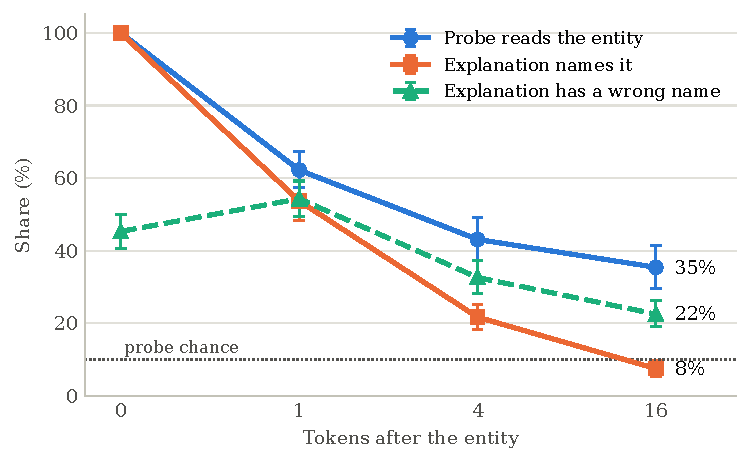
\includegraphics[width=0.78\linewidth]{fade}
\caption[The specific fades faster from the explanation than from the activation]{The specific fades faster
from the explanation than from the activation. Natural text, 540 held-out passages, four explanations per
activation; bars are 95\% intervals over entities. The dotted line is the probe's chance level; it does not
apply to the explanations, which are free text.}
\label{fig:fade}
\end{figure}

\begin{table}[t]
\centering
\footnotesize
\setlength{\tabcolsep}{4pt}
\begin{tabular}{@{}cllllc@{}}
\toprule
\shortstack[l]{Tokens after\\entity} & Probe reads it & \shortstack[l]{Names the true\\entity} & \shortstack[l]{At least one\\wrong name} & \shortstack[l]{Only wrong\\names} & \shortstack[l]{Wrong names\\per\\explanation} \\
\midrule
0 & 100.0 {\scriptsize[100.0, 100.0]} & 100.0 {\scriptsize[99.9, 100.0]} & 45.3 {\scriptsize[40.7, 49.9]} & 0.0 {\scriptsize[0.0, 0.1]} & 0.72 \\
1 & 62.2 {\scriptsize[57.4, 67.2]} & 53.7 {\scriptsize[48.3, 59.2]} & 54.3 {\scriptsize[49.5, 59.2]} & 25.1 {\scriptsize[21.5, 28.9]} & 1.10 \\
4 & 43.1 {\scriptsize[37.4, 49.1]} & 21.7 {\scriptsize[18.2, 25.2]} & 32.6 {\scriptsize[28.1, 37.3]} & 23.5 {\scriptsize[19.8, 27.2]} & 0.52 \\
16 & 35.4 {\scriptsize[29.6, 41.5]} & 7.5 {\scriptsize[5.4, 9.8]} & 22.5 {\scriptsize[19.0, 26.3]} & 20.0 {\scriptsize[16.7, 23.6]} & 0.33 \\
\bottomrule
\end{tabular}

\caption[What the explanations name]{What the explanations name, in \% of explanations with 95\% intervals.
Natural text, 540 passages, 8{,}640 explanations. ``Only wrong names'' means the explanation names a wrong
same-type entity and not the true one. The first column is the probe's accuracy on the same passages.}
\label{tab:names}
\end{table}

At distance~0 the two agree: the explanation names the entity in all but one of 2{,}160 cases. After that
they part. At 4 tokens the probe reads the entity 43\% of the time and the explanation names it 22\% of the
time. At 16 tokens it is 35\% against 7.5\%. The verbalizer is leaving on the table between half and four
fifths of what a simple linear reader can still get.

This comparison is somewhat unfair to the verbalizer: the probe must answer every time, while the verbalizer
can stay silent. Table~\ref{tab:fair} corrects for that by scoring the probe only on its most confident
passages, as many as the verbalizer chose to name something in.

\begin{table}[t]
\centering
\small
\begin{tabular}{@{}ccll@{}}
\toprule
\shortstack[l]{Tokens after\\entity} & \shortstack[l]{Names any\\same-type\\entity} & \shortstack[l]{Verbalizer\\precision} & \shortstack[l]{Probe, equally\\selective} \\
\midrule
0 & 100.0\% & 100.0 {\scriptsize[99.9, 100.0]} & 100.0 {\scriptsize[100.0, 100.0]} \\
1 & 78.9\% & 68.1 {\scriptsize[63.1, 72.9]} & 69.2 {\scriptsize[64.1, 74.0]} \\
4 & 45.2\% & 48.1 {\scriptsize[41.7, 54.4]} & 50.8 {\scriptsize[41.5, 60.9]} \\
16 & 27.5\% & 27.2 {\scriptsize[20.4, 34.2]} & 52.7 {\scriptsize[42.4, 63.4]} \\
\bottomrule
\end{tabular}

\caption[The verbalizer against an equally selective probe]{The verbalizer against an equally selective
probe (\%, 95\% intervals; natural text). Precision is the share of naming explanations that name the true
entity. The probe is scored on its most confident passages, as many as the verbalizer chose to name.}
\label{tab:fair}
\end{table}

At 1 and 4 tokens, when the verbalizer names something it is about as accurate as the equally selective
probe: 68\% against 69\%, and 48\% against 51\%. Its lower true-name rate there comes from speaking less
often, which is defensible. At 16
tokens the two separate: the verbalizer's precision is 27\%, the probe's is 53\%. Far from the entity, when
the verbalizer names something of the right type, it names the wrong thing three times out of four.

\section{Wrong Names}
\label{sec:wrongnames}

The orange line in Figure~\ref{fig:fade} falling would be harmless on its own. What makes it a problem is
the green line. At every distance a large share of explanations contain at least one wrong name of the
entity's type: 45\% at the entity's token, 54\% one token later, and still 22\% at 16 tokens
(Table~\ref{tab:names}).

Two things stand out. First, wrong names are common even at distance~0, where the true name is always
present. There the explanation typically names the right entity and then adds others around it. In one
example about a recording of Beethoven's Spring sonata, the explanation correctly quotes ``and Beethoven''
but also invents ``Mozart's complete piano sonatas'' as the preceding item. Second, as the true name
disappears the wrong names do not disappear with it. By 16 tokens, an explanation that names any entity of
the type is far more likely to be naming only a wrong one (20\% of all explanations) than the true one
(7.5\%).

The wrong names are not drawn from my list of 60. At 4 tokens, 77\% of them are same-type entities outside
the list, and at 16 tokens 82\%. The most common are everyday members of the type: guitar, dog, piano and
lion at 4 tokens; Toronto, piano, guitar and Italy at 16. They look like what one would guess knowing only
the type. Here is a typical case, four tokens after \emph{Moscow}:

\begin{sample}{Passage (read to four tokens past \emph{Moscow})}
\ldots At nine, Forough was the youngest ever to be admitted to the Royal Conservatory of Music, Brussels as
a pupil of Arthur Grumiaux. Later studies were with David Oistrakh at the \true{Moscow} Conservatory. \ldots
\end{sample}

\begin{sample}{Explanation}
Wikipedia biographical article format with English language entries on Ukrainian tenor Vladimir Ashkenazy,
detailing career and musical achievements. The sentence structure ``Ashkenazy studied music in
\wrong{Paris} beginning in 1952, and won international competitions \ldots''
\end{sample}

The gist is intact: a biography of a classical musician with Soviet connections, studying at a conservatory
in a capital city. The city is wrong, and so is the musician.

\section{Name Position}

Each explanation describes the context and then predicts what comes next. A wrong name in the prediction
(``expecting \emph{Paris} or \emph{London}'') is a guess labelled as a guess. A wrong name in the description
of the context is a false statement about what the model read. Table~\ref{tab:position} separates the two,
cutting each explanation at the phrase that introduces its predicted continuation.

\begin{table}[t]
\centering
\small
\setlength{\tabcolsep}{5pt}
\begin{tabular}{@{}cllll@{}}
\toprule
\shortstack[l]{Tokens after\\entity} & \shortstack[l]{True name,\\context} & \shortstack[l]{True name,\\continuation} & \shortstack[l]{Wrong name,\\context} & \shortstack[l]{Wrong name,\\continuation} \\
\midrule
0 & 100.0 {\scriptsize[99.9, 100.0]} & 11.1 {\scriptsize[8.1, 14.6]} & 35.8 {\scriptsize[32.2, 39.4]} & 17.9 {\scriptsize[14.5, 21.5]} \\
1 & 53.1 {\scriptsize[47.5, 58.6]} & 7.8 {\scriptsize[5.9, 9.8]} & 51.7 {\scriptsize[47.0, 56.4]} & 15.3 {\scriptsize[12.5, 18.2]} \\
4 & 20.5 {\scriptsize[17.0, 24.0]} & 3.2 {\scriptsize[2.0, 4.5]} & 30.2 {\scriptsize[26.0, 34.6]} & 7.7 {\scriptsize[6.0, 9.5]} \\
16 & 6.7 {\scriptsize[4.7, 8.8]} & 1.4 {\scriptsize[0.7, 2.1]} & 20.8 {\scriptsize[17.4, 24.4]} & 4.8 {\scriptsize[3.5, 6.2]} \\
\bottomrule
\end{tabular}

\caption[Where names sit in the explanation]{Where names sit in the explanation: \% of explanations with a
true or wrong name in the part that describes the context, and in the part that predicts the continuation.
Natural text; 95\% intervals.}
\label{tab:position}
\end{table}

Most wrong names are in the description, not the prediction. One token after the entity, 52\% of
explanations have a wrong name in the context part and 15\% have one in the continuation part; in raw
counts, 1{,}993 wrong names against 495. The ratio is between two and five to one at every distance. The problem is
therefore not that the verbalizer hedges with a list of candidates for the next word. It states, as a
description of the text, things that are not in the text.

In short, the specific fades faster from the explanation than from the activation, and what takes its place
is a plausible wrong name stated as fact.

\chapter{Incentives}
\label{ch:incentives}

The verbalizer was trained to maximise one number, the reconstruction cosine. If wrong names cost it
nothing, training never had a reason to remove them. This chapter tests that directly.

\section{Edit Test}

I took explanations at distances 0 and 1 that name the true entity and also contain at least one wrong name
in the part describing the context. There are 1{,}352 of them; I sampled 1{,}000. For each I made two edited
copies and sent all three through the reconstructor.

\begin{itemize}
\item \textbf{Wrong names removed.} Every wrong same-type name is replaced by a neutral phrase such as
``another city''. The true name stays.
\item \textbf{True name removed.} The true name is replaced the same way. The wrong names stay. This is the
control: it shows what an edit of the same size costs when it removes real information.
\end{itemize}

Writing $z^{-W}$ for the copy with wrong names removed and $z^{-e}$ for the copy with the true name removed,
the quantities of interest are what each kind of name is worth to the score of Equation~\ref{eq:score}:
\begin{equation}
\Delta_{\text{wrong}} = s(h,z) - s(h,z^{-W}), \qquad \Delta_{\text{true}} = s(h,z) - s(h,z^{-e}).
\label{eq:delta}
\end{equation}
If $\Delta_{\text{wrong}} \le 0$, the objective in Equation~\ref{eq:objective} would already discourage wrong
names. If it is near zero or positive, it does not.

The edits worked as intended: afterwards no wrong name is detected in 99.8\% of the first copies, and the
true name is gone from 94.3\% of the second.

\section{Results}

\begin{table}[t]
\centering
\footnotesize
\setlength{\tabcolsep}{3.5pt}
\resizebox{\linewidth}{!}{\begin{tabular}{@{}crlllll@{}}
\toprule
\shortstack[l]{Tokens after\\entity} & $n$ & Original & \shortstack[l]{Wrong names\\removed} & \shortstack[l]{True name\\removed} & \shortstack[l]{Original beats\\``wrong\\removed''} & \shortstack[l]{Original beats\\``true\\removed''} \\
\midrule
0 & 567 & 0.897 {\scriptsize[0.892, 0.902]} & 0.894 {\scriptsize[0.889, 0.899]} & 0.686 {\scriptsize[0.676, 0.695]} & 67.5 {\scriptsize[63.0, 72.1]} & 100.0 {\scriptsize[100.0, 100.0]} \\
1 & 433 & 0.895 {\scriptsize[0.886, 0.903]} & 0.889 {\scriptsize[0.880, 0.897]} & 0.879 {\scriptsize[0.869, 0.887]} & 79.9 {\scriptsize[75.5, 84.2]} & 88.2 {\scriptsize[84.1, 92.0]} \\
0 and 1 & 1{,}000 & 0.896 {\scriptsize[0.890, 0.901]} & 0.892 {\scriptsize[0.886, 0.897]} & 0.769 {\scriptsize[0.759, 0.779]} & 72.9 {\scriptsize[69.6, 76.1]} & 94.9 {\scriptsize[93.1, 96.6]} \\
\bottomrule
\end{tabular}
}
\caption[Reconstruction cosine before and after editing names out]{Reconstruction cosine before and after
editing names out, and how often the original scores higher than each edit (\%). Natural text; 95\%
intervals over passages.}
\label{tab:edit}
\end{table}

\begin{figure}[t]
\centering
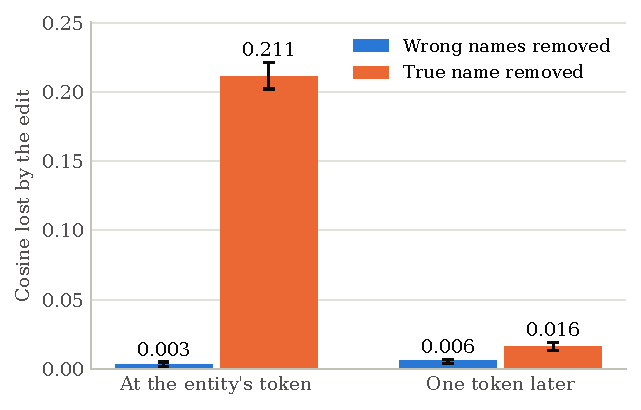
\includegraphics[width=0.6\linewidth]{edit}
\caption[What each kind of name is worth to the reconstruction score]{What each kind of name is worth to
the reconstruction score: cosine lost when it is edited out. Natural text; 95\% intervals.}
\label{fig:edit}
\end{figure}

$\Delta_{\text{wrong}}$ is 0.003 at the entity's token and 0.006 one token later (Table~\ref{tab:edit},
Figure~\ref{fig:edit}); per name removed, about 0.002. $\Delta_{\text{true}}$ is 0.211 at the entity's
token, seventy times as much, and 0.016 one token later.

\section{Interpretation}

Three things follow.

\textbf{Wrong names are nearly free, and slightly rewarded.} The original beats the cleaned copy 68\% of the
time at distance~0 and 80\% at distance~1. A wrong but plausible name of the right type reconstructs a
little better than a vague phrase, presumably because it still tells the reconstructor the type and the
topic. So the objective gives the verbalizer a small push towards naming \emph{something}.

\textbf{The true name stops mattering quickly.} It is worth 0.21 while the model is reading it and 0.016 a
single token later. From then on, getting the specific right earns almost nothing, so a verbalizer trained
only on reconstruction has little reason to keep track of it.

\textbf{This sets the scale for a fix.} A penalty of $\lambda$ per suspect name changes the reward to
$s(h,z) - \lambda\,|U(z)|$, where $U(z)$ is the set of names to discourage. For it to bite without also
driving out true names, $\lambda$ must sit between what a wrong name earns and what a true one earns:
\begin{equation}
0.002 \;\approx\; \Delta_{\text{wrong}} \text{ per name} \;<\; \lambda \;<\; \Delta_{\text{true}} \;\approx\; 0.016
\text{ (one token after the entity).}
\end{equation}
The fine-tuning experiments use $\lambda = 0.01$.

The verbalizer is doing what an autoencoder does: it keeps what helps reconstruction. The specific helps
very little, so nothing protects it.

\chapter{Agreement}
\label{ch:agreement}

If the reconstruction score cannot tell a true name from a wrong one, something else must. This chapter
shows that the verbalizer's own samples can: a name it writes every time is usually true, and a name it
writes once is usually not.

\section{Consensus}

Each activation has $K=4$ independently sampled explanations $z_1,\dots,z_K$. For every name $n$ that appears
in any of them, I count how many contain it:
\begin{equation}
c(n) = \sum_{k=1}^{K} \mathbf{1}\bigl[\, n \in N(z_k) \,\bigr].
\label{eq:count}
\end{equation} Figure~\ref{fig:consensus} shows how often a name is true at each
count, pooling distances 1, 4 and 16. Distance~0 is left out of the pooled figure because the true name is
always present there, which would flatter the result.

\begin{figure}[t]
\centering
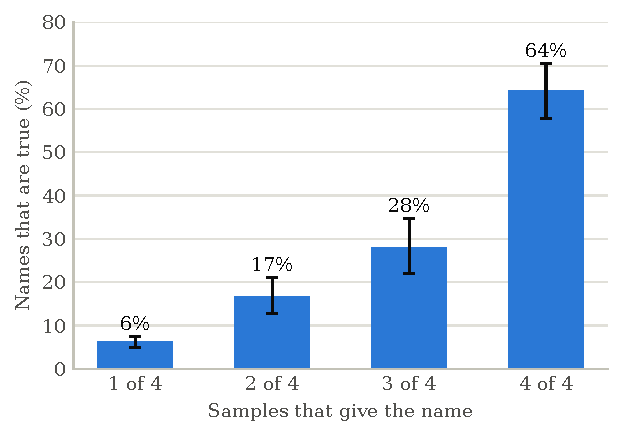
\includegraphics[width=0.6\linewidth]{consensus}
\caption[Names that more samples agree on are more often true]{Names that more samples agree on are more
often true. Natural text, distances 1, 4 and 16 pooled, 3{,}489 names; 95\% intervals.}
\label{fig:consensus}
\end{figure}

A name given by one sample is true 6\% of the time. A name given by all four is true 64\% of the time. As a
score for ranking names, the agreement count has an AUC of 0.80, and it holds up at every distance
(Table~\ref{tab:consensus}).

\begin{table}[t]
\centering
\footnotesize
\setlength{\tabcolsep}{4pt}
\begin{tabular}{@{}lllll@{}}
\toprule
\shortstack[l]{Tokens after\\entity} & 1 of 4 & 2 of 4 & 3 of 4 & 4 of 4 \\
\midrule
0 & 0.0 {\scriptsize[0.0, 0.0]} (717) & 0.0 {\scriptsize[0.0, 0.0]} (148) & 1.3 {\scriptsize[0.0, 3.8]} (78) & 87.5 {\scriptsize[84.8, 90.3]} (616) \\
1 & 5.2 {\scriptsize[3.8, 6.8]} (1{,}113) & 14.2 {\scriptsize[10.1, 18.4]} (240) & 20.3 {\scriptsize[14.1, 27.3]} (182) & 66.4 {\scriptsize[59.7, 73.0]} (348) \\
4 & 7.8 {\scriptsize[5.9, 10.0]} (667) & 20.0 {\scriptsize[11.5, 30.0]} (115) & 39.3 {\scriptsize[28.9, 50.7]} (84) & 62.4 {\scriptsize[53.0, 71.7]} (109) \\
16 & 6.1 {\scriptsize[4.1, 8.5]} (478) & 19.3 {\scriptsize[11.4, 28.4]} (83) & 39.0 {\scriptsize[21.4, 57.9]} (41) & 44.8 {\scriptsize[26.9, 62.1]} (29) \\
1, 4 and 16 & 6.2 {\scriptsize[5.0, 7.5]} (2{,}258) & 16.7 {\scriptsize[12.7, 21.1]} (438) & 28.0 {\scriptsize[22.0, 34.8]} (307) & 64.2 {\scriptsize[57.7, 70.5]} (486) \\
\bottomrule
\end{tabular}

\caption[Precision of a name by how many samples give it]{Precision of a name (\%) by how many of the four
samples give it, with the number of names in brackets. Natural text; 95\% intervals.}
\label{tab:consensus}
\end{table}

\section{Filter}

This suggests a filter that needs no training: keep a name only if $c(n) \ge m$ for some threshold $m$. Table~\ref{tab:filter} shows the trade-off in the terms of retrieval, treating the names as
retrieved items.

\begin{table}[t]
\centering
\small
\begin{tabular}{@{}lllll@{}}
\toprule
\shortstack[l]{Keep a name if\\given by} & \shortstack[l]{Wrong names\\removed} & \shortstack[l]{True names\\kept} & Precision & Names left \\
\midrule
None & 0 & 100 & 17.5 {\scriptsize[15.1, 20.1]} & 3{,}489 \\
At least 2 of 4 & 73.6 {\scriptsize[69.9, 77.3]} & 77.2 {\scriptsize[73.5, 80.6]} & 38.3 {\scriptsize[33.5, 43.4]} & 1{,}231 \\
At least 3 of 4 & 86.3 {\scriptsize[83.9, 88.6]} & 65.2 {\scriptsize[61.6, 68.9]} & 50.2 {\scriptsize[44.6, 56.2]} & 793 \\
All 4 & 94.0 {\scriptsize[92.7, 95.2]} & 51.1 {\scriptsize[46.3, 55.9]} & 64.2 {\scriptsize[57.7, 70.5]} & 486 \\
\bottomrule
\end{tabular}

\caption[The agreement filter as a precision--recall trade-off]{The agreement filter as a
precision--recall trade-off (\%). Natural text, distances 1, 4 and 16 pooled; 95\% intervals. ``True names
kept'' is recall relative to no filter.}
\label{tab:filter}
\end{table}

Requiring two of four removes 74\% of the wrong names and keeps 77\% of the true ones, which doubles
precision from 17.5\% to 38\%. Requiring all four reaches 64\% precision but keeps only half the true names.
Two of four is the setting I carry forward: it removes most of the damage for a modest loss.

The cost is compute. Four explanations instead of one is four times the generation. The filter also only
removes names; it cannot recover a true name the verbalizer never wrote.

\section{Verifiers}

Agreement uses only the verbalizer's outputs. An alternative is to check each name against the activation
itself: does the activation point towards the named entity more than towards its rivals?
Table~\ref{tab:verifiers} compares three such checks.

\begin{table}[t]
\centering
\small
\begin{tabular}{@{}clll@{}}
\toprule
\shortstack[l]{Tokens after\\entity} & \shortstack[l]{Concept\\vectors} & \shortstack[l]{Probe\\directions} & \shortstack[l]{Agreement\\count} \\
\midrule
0 & 0.79 {\scriptsize[0.74, 0.84]} & 1.00 {\scriptsize[1.00, 1.00]} & 0.96 {\scriptsize[0.95, 0.97]} \\
1 & 0.69 {\scriptsize[0.63, 0.74]} & 0.90 {\scriptsize[0.86, 0.92]} & 0.83 {\scriptsize[0.80, 0.86]} \\
4 & 0.66 {\scriptsize[0.57, 0.73]} & 0.76 {\scriptsize[0.69, 0.84]} & 0.77 {\scriptsize[0.74, 0.80]} \\
16 & 0.65 {\scriptsize[0.54, 0.76]} & 0.70 {\scriptsize[0.61, 0.78]} & 0.72 {\scriptsize[0.66, 0.78]} \\
\bottomrule
\end{tabular}

\caption[Three ways to tell true names from wrong ones]{Three ways to tell true names from wrong ones (AUC,
95\% intervals; natural text). The first two score a name by the activation's similarity to a direction for
that entity; they cover only names among the 60 listed entities, so the columns are not computed on
identical sets of names.}
\label{tab:verifiers}
\end{table}

\begin{itemize}
\item \textbf{Concept vectors} are entity directions built without any labelled passages, from the target
model's activations on the prompt ``Tell me about X''. They are weak: AUC 0.65 to 0.79.
\item \textbf{Probe directions} come from the trained probe. They are the best check near the entity (0.90
at one token), but they need dozens of labelled passages for every entity one wants to verify.
\item \textbf{Agreement} needs neither labels nor access to the target model. It matches the probe
directions from four tokens on (0.77 against 0.76, and 0.72 against 0.70).
\end{itemize}

For a method whose selling point is that it is unsupervised, agreement is the natural check: it is nearly as
good as the supervised one and works for any name, not just the entities someone trained a probe for.

\chapter{Fine-tuning}
\label{ch:finetuning}

Chapter~\ref{ch:incentives} explained wrong names by the training objective: they cost nothing, so nothing
removes them. An explanation like that should survive an intervention. This chapter changes what the
verbalizer is rewarded for and checks that its behaviour changes the way the explanation predicts.

\section{Training Loop}

The loop is the simplest form of reward-driven training (Figure~\ref{fig:loop}). For each activation $h_i$, the current verbalizer
samples $K=8$ explanations. A score picks the best one,
\begin{equation}
z_i^{*} = \arg\max_{k}\; \mathrm{score}(h_i, z_{i,k}),
\end{equation}
and a low-rank adapter (LoRA~\cite{hu2022lora}) on the verbalizer is trained to make the chosen explanations
more likely, $\min_\theta -\sum_i \log V_\theta(z_i^{*} \mid h_i)$. The next round samples from the updated
verbalizer. The target model and the reconstructor stay frozen.

\begin{figure}[t]
\centering
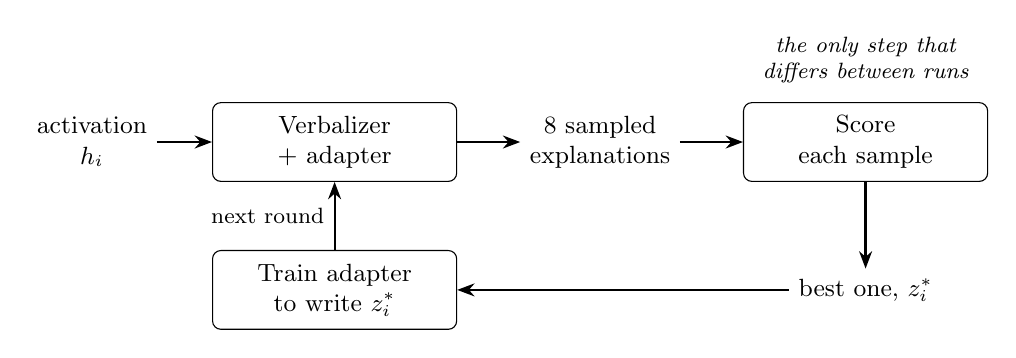
\begin{tikzpicture}[font=\small,
  box/.style={draw, rounded corners=3pt, minimum height=1.0cm, minimum width=3.1cm, align=center},
  data/.style={align=center},
  arr/.style={-{Stealth[length=2.2mm]}, thick}]
\node[data] (h) {activation\\$h_i$};
\node[box, right=0.7cm of h] (av) {Verbalizer\\+ adapter};
\node[data, right=0.8cm of av] (zs) {8 sampled\\explanations};
\node[box, right=0.8cm of zs] (sc) {Score\\each sample};
\node[data, below=1.1cm of sc] (best) {best one, $z_i^{*}$};
\node[box] (tr) at (av |- best) {Train adapter\\to write $z_i^{*}$};
\draw[arr] (h) -- (av);
\draw[arr] (av) -- (zs);
\draw[arr] (zs) -- (sc);
\draw[arr] (sc) -- (best);
\draw[arr] (best) -- (tr);
\draw[arr] (tr) -- node[left, font=\footnotesize]{next round} (av);
\node[font=\footnotesize\itshape, above=0.12cm of sc, align=center] {the only step that\\differs between runs};
\end{tikzpicture}
\caption[One round of the training loop]{One round of the training loop. The target model and the
reconstructor are frozen; only the adapter on the verbalizer is trained.}
\label{fig:loop}
\end{figure}

Each run uses 2{,}000 activations drawn from the 4{,}200 non-test passages at distances 0, 1, 4 and 16, and
runs three rounds. The first round's samples come from the released verbalizer and are shared by every run,
so the runs differ only in the score.

\section{Scores}

Four scores are compared. With $s$ the reconstruction score of Equation~\ref{eq:score}:

\begin{description}
\item[Reconstruction.] $\mathrm{score} = s(h,z)$. More of the original objective. This is the control: if
wrong names are free under $s$, it should not remove them.
\item[Lineup.] The reconstruction must pick $h$ out of a lineup of four: $h$ and three near-twins, obtained
by swapping the entity in the passage for another of its type. The score is the log-probability of picking
$h$ under a softmax over the four cosines. This is still reconstruction, made sensitive to the specific.
\item[Hold back.] $\mathrm{score} = s(h,z) - \lambda\,|U(z)|$ with $\lambda = 0.01$, where $U(z)$ is the set of
names in $z$ that fewer than two of the released verbalizer's other samples for the same activation also
give. This adds the missing cost on unsupported names, using only the agreement signal of
Chapter~\ref{ch:agreement}. No labels are involved.
\item[Keep the specific.] Hold back, plus a bonus of 0.05 when $z$ names the entity that is really in the
passage. This one uses the passage as a label. It asks a different question: can the verbalizer be taught to
\emph{recover} the specific, not just to stop inventing one? To separate reading from memorising, twelve
entities (two per type) are kept out of its training.
\end{description}

\section{Results}

Every fine-tuned verbalizer is evaluated like the released one: the same 540 held-out passages, four
distances, four samples. Differences are paired per entity.

\begin{table}[t]
\centering
\small
\begin{tabular}{@{}llrl@{}}
\toprule
Score & \shortstack[l]{Change in\\wrong names\\per\\explanation} & Relative & \shortstack[l]{Change in\\true-name rate\\(points)} \\
\midrule
Reconstruction & $-$0.008 {\scriptsize[$-$0.028, $+$0.011]} & $-$1.3\% & $+$0.0 {\scriptsize[$-$0.5, $+$0.6]} \\
Lineup & $-$0.003 {\scriptsize[$-$0.022, $+$0.015]} & $-$0.5\% & $-$0.3 {\scriptsize[$-$0.9, $+$0.2]} \\
Hold back & $-$0.056 {\scriptsize[$-$0.080, $-$0.031]} & $-$8.4\% & $-$0.2 {\scriptsize[$-$0.8, $+$0.4]} \\
Hold back, second run & $-$0.034 {\scriptsize[$-$0.055, $-$0.012]} & $-$5.1\% & $-$0.1 {\scriptsize[$-$0.8, $+$0.5]} \\
Keep the specific & $-$0.019 {\scriptsize[$-$0.039, $+$0.001]} & $-$2.9\% & $+$0.2 {\scriptsize[$-$0.4, $+$0.8]} \\
\bottomrule
\end{tabular}

\caption[Fine-tuned verbalizers against the released one]{Fine-tuned verbalizers against the released one,
all four distances pooled. Natural text, 540 held-out passages; 95\% intervals from a paired bootstrap over
entities. The released verbalizer has 0.667 wrong names per explanation and a true-name rate of 45.7\%.}
\label{tab:arms}
\end{table}

\begin{figure}[t]
\centering
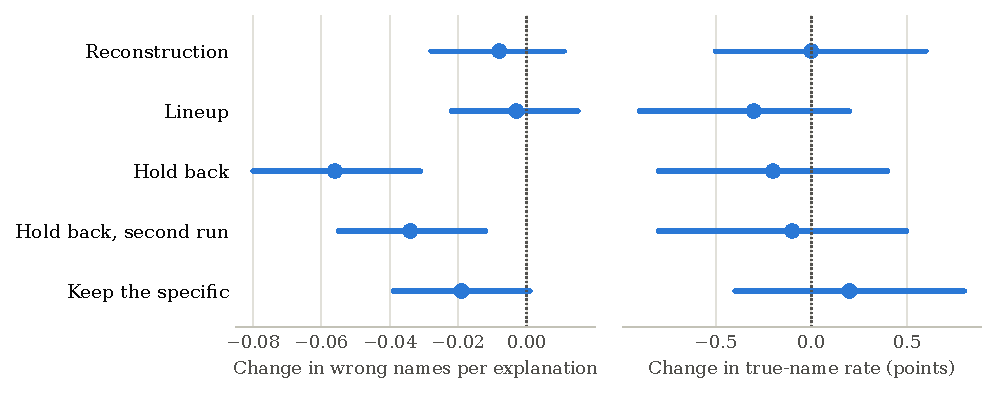
\includegraphics[width=0.92\linewidth]{arms}
\caption[Only the penalty on unsupported names moves wrong names]{Only the penalty on unsupported names
moves wrong names, in both runs, and nothing moves true names. Change relative to the released verbalizer; lines are 95\%
intervals. Natural text, held-out passages.}
\label{fig:arms}
\end{figure}

Both predictions hold (Table~\ref{tab:arms}, Figure~\ref{fig:arms}).

\textbf{More reconstruction changes nothing.} Three further rounds on the original objective leave wrong
names where they were ($-1.3\%$, interval spanning zero). Making reconstruction harder with the lineup does
not help either ($-0.5\%$).

\textbf{A cost on unsupported names removes some of them.} Hold back cuts wrong names by 8.4\%, with an
interval well clear of zero. A second run from a different seed, with its own training passages and
samples, cuts them by 5.1\%, again clear of zero. In both runs the true-name rate, the reconstruction cosine
and the length of the explanations are unchanged, so the verbalizer has not simply learned to name less.

\textbf{The specific cannot be coaxed back.} Rewarding the true name does not raise the true-name rate: $+0.2$
points overall, and $-0.7$ points on the entities held out of training (Table~\ref{tab:keep}). The samples it
was trained on named the true entity 56\% of the time against 45\% on average, yet the trained verbalizer
stays at 45\%.

\begin{table}[t]
\centering
\small
\begin{tabular}{@{}lll@{}}
\toprule
Entities & \shortstack[l]{Change in\\true-name rate\\(points)} & \shortstack[l]{Change in\\wrong names\\per\\explanation} \\
\midrule
Trained on (48) & $+$0.5 {\scriptsize[$-$0.2, $+$1.1]} & $-$0.017 {\scriptsize[$-$0.039, $+$0.006]} \\
Held out of training (12) & $-$0.7 {\scriptsize[$-$2.2, $+$0.9]} & $-$0.028 {\scriptsize[$-$0.072, $+$0.014]} \\
\bottomrule
\end{tabular}

\caption[Keep the specific, by whether the entity was seen in training]{The keep-the-specific verbalizer
against the released one, split by whether the entity was seen in training. Natural text, held-out
passages; 95\% intervals.}
\label{tab:keep}
\end{table}

\section{Analysis}

\textbf{Why the hold-back effect is small.} The samples chosen for training had 35\% fewer wrong names than
average; the trained verbalizer writes 5 to 8\% fewer. Imitating a slightly better subset of one's own samples is
a weak push, because the verbalizer already finds those samples likely. Training harder on the same samples
does not help: five passes over the first round's choices fit them far more closely but gave a smaller
held-out effect ($-6.5\%$), which is memorisation.

\textbf{Why the specific does not come back.} When one of eight samples names the right entity far from it,
that sample looks like a lucky draw, not a skill. A skill would transfer to new passages after training; a
lucky draw does not. This fits Chapter~\ref{ch:fading}: at
16 tokens the information the probe reads is real, but the verbalizer has no reliable way to reach it.
Dingeto~\cite{dingeto2026recap} reports the same for a direct truth reward in a different setting.

\textbf{Filter or fine-tune?} Table~\ref{tab:combine} puts the two fixes side by side. The agreement filter
alone removes 44 to 62\% of the wrong names, depending on distance. Hold back removes 5 to 8\% overall. Together
they are only slightly better than the filter alone.

\begin{table}[t]
\centering
\footnotesize
\setlength{\tabcolsep}{4pt}
\begin{tabular}{@{}cllll@{}}
\toprule
\shortstack[l]{Tokens after\\entity} & Released & Hold back & \shortstack[l]{Released,\\filtered} & \shortstack[l]{Hold back,\\filtered} \\
\midrule
0 & 0.719 {\scriptsize[0.627, 0.813]} & 0.667 {\scriptsize[0.584, 0.755]} & 0.387 {\scriptsize[0.321, 0.454]} & 0.360 {\scriptsize[0.304, 0.416]} \\
1 & 1.097 {\scriptsize[0.954, 1.249]} & 1.006 {\scriptsize[0.876, 1.143]} & 0.609 {\scriptsize[0.508, 0.715]} & 0.554 {\scriptsize[0.463, 0.650]} \\
4 & 0.517 {\scriptsize[0.432, 0.605]} & 0.462 {\scriptsize[0.382, 0.547]} & 0.232 {\scriptsize[0.182, 0.283]} & 0.210 {\scriptsize[0.163, 0.263]} \\
16 & 0.334 {\scriptsize[0.268, 0.409]} & 0.309 {\scriptsize[0.250, 0.373]} & 0.126 {\scriptsize[0.099, 0.156]} & 0.119 {\scriptsize[0.088, 0.150]} \\
\bottomrule
\end{tabular}

\caption[The filter and fine-tuning compared]{Wrong names per explanation with fine-tuning (the first hold-back run),
with the two-of-four agreement filter, and with both. Natural text, held-out passages; 95\% intervals.}
\label{tab:combine}
\end{table}

Larger changes to training, such as a grounding reward~\cite{hong2026grounding} or a different
reconstruction objective~\cite{lek2026flownla}, may well do more. The fine-tuning here matters less as a fix
than as a test. The account in Chapter~\ref{ch:incentives} said what
would happen under each reward, and that is what happened.

\chapter{Conclusion}
\label{ch:conclusion}

\section{Takeaways}

An NLA explanation should be read as two things of different reliability. The gist is what the
reconstruction objective pays for, and it is usually right. A specific name is something the objective
hardly prices at all once the model has moved past the token, so the verbalizer supplies one that fits the
gist. Far from the entity, a name in an explanation is wrong about three times in four.

The verbalizer does, however, know which of its names are shaky. Its own token probabilities separate true
names from wrong ones, and agreement between a few samples does so a little better. Training on that signal
removes some wrong names; training on reconstruction removes none; and no reward tried here brings a lost
specific back.

For someone using an NLA today, the advice is short: trust the gist, and do not trust a name unless several
samples agree on it.

\section{Limitations}
\label{ch:limitations}

\textbf{One model, one layer.} Everything is measured on the released NLA for Qwen2.5-7B at layer~20. The
argument about incentives is general, but the numbers are not, and NLAs for larger models may fade more
slowly.

\textbf{Sixty entities.} The entities are common ones, on Wikipedia text. Rare entities, numbers, dates and
other kinds of specific are untested.

\textbf{The name detector.} Its accuracy has not been measured on a labelled sample, only inspected by hand
on 30 cases. Every comparison uses the same detector, so differences between conditions are safer than
absolute rates.

\textbf{The probe.} It is a floor on what the activation holds, and it chooses among ten known answers while
the verbalizer writes free text. The gap between them is therefore an estimate, not a measurement, of what
the verbalizer leaves unsaid.

\textbf{Small training runs.} Each fine-tuning run uses 2{,}000 activations and a few hundred gradient steps.
A longer run, or true policy-gradient training as the authors used, might move the verbalizer further than
the 8\% seen here.

\section{Next Steps}

The cleanest follow-up is to put the cost on wrong names into the original training, not a small fine-tune
after it: add the agreement penalty to the reward during the authors' reinforcement-learning stage and see
whether the fade in Chapter~\ref{ch:fading} narrows towards the probe. The second is to expose the
confidence the verbalizer already has, by marking low-probability names in the explanation itself.


\bibliographystyle{plainnat}
\bibliography{refs}

\appendix
\chapter{Reproducibility}
\label{app:repro}

The code, the explanations and the result tables are in the GitHub repository; the fine-tuned adapters, the
activations and the cached reconstructions are on Hugging Face (links in Section~\ref{sec:availability}).
\texttt{fetch\_artifacts.py} downloads the large files into place.

\begin{table}[h]
\centering
\small
\setlength{\tabcolsep}{4pt}
\begin{tabular}{@{}ll@{}}
\toprule
Result & Command \\
\midrule
Chapter~\ref{ch:fading}: fade curve, probe, names & \texttt{python fade\_curve.py} \\
Chapters~\ref{ch:fading}, \ref{ch:agreement}: positions, agreement, filter & \texttt{python name\_analysis.py} \\
Chapter~\ref{ch:incentives}: edit test & \texttt{python edit\_test.py} \\
Chapter~\ref{ch:agreement}: confidence & \texttt{python confidence.py} \\
Chapter~\ref{ch:finetuning}: training & \texttt{python finetune.py configs/holdback.json} \\
Chapter~\ref{ch:finetuning}: evaluation & \texttt{python evaluate.py <adapter>} \\
Chapter~\ref{ch:finetuning}: paired comparison & \texttt{python compare.py <names>} \\
Every table and figure here & \texttt{python paper/build\_assets.py} \\
\bottomrule
\end{tabular}
\caption{Which script produces which result.}
\end{table}

All but training and evaluation run on a laptop from the saved files. Seeds are fixed throughout.

\section{Hardware}

Three machines were used (Table~\ref{tab:hardware}). The models run in 16-bit precision on all of them.

\begin{table}[h]
\centering
\footnotesize
\setlength{\tabcolsep}{4pt}
\begin{tabular}{@{}p{0.2\linewidth}p{0.27\linewidth}p{0.3\linewidth}p{0.15\linewidth}@{}}
\toprule
Machine & Specification & Used for & Precision \\
\midrule
Laptop & MacBook Air, Apple M5, 10 cores, 24\,GB memory, macOS 26.6 & Extracting activations, probes, every analysis and table & bfloat16 (MPS) \\
Kaggle notebook & 2 $\times$ NVIDIA Tesla T4, 15\,GB each & Pipeline check; generating the 8{,}640 explanations (batch 32, 70 per minute, 123 minutes) & float16 \\
Rented GPU & 1 $\times$ NVIDIA RTX A6000, 48\,GB; 16 virtual CPUs, 62\,GB memory & Reconstruction run; evaluating the released and reconstruction verbalizers & bfloat16 \\
Rented GPUs & 2 $\times$ NVIDIA A40, 48\,GB, one run per card & All other fine-tuning runs and evaluations; token probabilities & bfloat16 \\
\bottomrule
\end{tabular}
\caption{Hardware.}
\label{tab:hardware}
\end{table}

On the 48\,GB cards generation ran at batch 128, about 800 to 900 explanations per minute. Fine-tuning peaked
at 44\,GB of GPU memory, and a three-round run with its evaluation took about 100 minutes.

\section{Software}

\begin{table}[h]
\centering
\footnotesize
\setlength{\tabcolsep}{4pt}
\begin{tabular}{@{}lll@{}}
\toprule
 & Laptop & Rented GPUs \\
\midrule
Python & 3.12.13 & 3.12 \\
PyTorch & 2.15.0 & 2.8.0 with CUDA 12.8 (Ubuntu 24.04) \\
transformers & 4.57.6 & 4.57 \\
peft & 0.21.2 & 0.21.2 \\
scikit-learn, spaCy, NLTK & 1.9.1, 3.8.18, 3.10.4 & same \\
\bottomrule
\end{tabular}
\caption[Software versions]{Software versions. The Kaggle notebook used PyTorch 2.11.0 with the same
transformers range. \texttt{requirements.txt} pins the laptop environment.}
\label{tab:software}
\end{table}

The three models are fixed to these revisions on Hugging Face:
{\small
\begin{itemize}
\item target model, \texttt{Qwen/Qwen2.5-7B-Instruct}, revision \texttt{a09a3545}
\item verbalizer, \texttt{kitft/nla-qwen2.5-7b-L20-av}, revision \texttt{b8846916}
\item reconstructor, \texttt{kitft/nla-qwen2.5-7b-L20-ar}, revision \texttt{e2c9e57e}
\end{itemize}}
Fine-tuning used a LoRA of rank 16
(scale 32, dropout 0.05) on the four attention projections, AdamW with learning rate $10^{-4}$, batch size 8
and one pass over the chosen explanations per round.

\chapter{Layer Indexing}
\label{app:layer}

The NLA for Qwen2.5-7B is trained on ``layer 20'', meaning the output of transformer block 20. In the
Hugging Face convention \texttt{hidden\_states[0]} is the embedding output, so the output of block 20 is
\texttt{hidden\_states[21]}. The usage example published with the models reads \texttt{hidden\_states[20]},
one block early.

Nothing fails when this happens. The explanations still read sensibly, because neighbouring layers are
similar. Only the numbers give it away: on the same passages, reading one block early gave a mean cosine of
0.846 and an activation norm of 95.7, against 0.893 and 112.7 at the right layer, and the reference norm
for this layer is 111.3. I found the error when the first check against a known reconstruction quality came
out low, and all results in this report use the corrected layer.

\chapter{Full Tables}
\label{app:tables}

\begin{table}[h]
\centering
\footnotesize
\setlength{\tabcolsep}{4pt}
\begin{tabular}{@{}llllll@{}}
\toprule
\shortstack[l]{Tokens after\\entity} & \shortstack[l]{Keep a name if\\given by} & \shortstack[l]{Wrong names\\removed} & \shortstack[l]{True names\\kept} & Precision & Names left \\
\midrule
0 & None & 0 & 100 & 34.6 {\scriptsize[32.0, 37.5]} & 1{,}559 \\
0 & At least 2 of 4 & 70.4 {\scriptsize[66.6, 74.0]} & 100.0 {\scriptsize[100.0, 100.0]} & 64.1 {\scriptsize[60.5, 68.1]} & 842 \\
0 & At least 3 of 4 & 84.9 {\scriptsize[82.5, 87.2]} & 100.0 {\scriptsize[100.0, 100.0]} & 77.8 {\scriptsize[74.5, 81.3]} & 694 \\
0 & All 4 & 92.4 {\scriptsize[90.8, 94.0]} & 99.8 {\scriptsize[99.4, 100.0]} & 87.5 {\scriptsize[84.8, 90.3]} & 616 \\
1 & None & 0 & 100 & 19.1 {\scriptsize[16.7, 21.8]} & 1{,}883 \\
1 & At least 2 of 4 & 69.3 {\scriptsize[65.4, 73.0]} & 83.9 {\scriptsize[79.8, 87.6]} & 39.2 {\scriptsize[34.4, 44.3]} & 770 \\
1 & At least 3 of 4 & 82.8 {\scriptsize[80.0, 85.5]} & 74.4 {\scriptsize[69.7, 79.0]} & 50.6 {\scriptsize[45.0, 56.3]} & 530 \\
1 & All 4 & 92.3 {\scriptsize[90.7, 93.9]} & 64.2 {\scriptsize[57.9, 70.1]} & 66.4 {\scriptsize[59.7, 73.0]} & 348 \\
4 & None & 0 & 100 & 18.1 {\scriptsize[15.0, 21.7]} & 975 \\
4 & At least 2 of 4 & 77.0 {\scriptsize[72.7, 81.1]} & 70.5 {\scriptsize[64.2, 76.5]} & 40.3 {\scriptsize[33.5, 47.7]} & 308 \\
4 & At least 3 of 4 & 88.5 {\scriptsize[85.7, 91.1]} & 57.4 {\scriptsize[52.1, 63.0]} & 52.3 {\scriptsize[44.7, 60.5]} & 193 \\
4 & All 4 & 94.9 {\scriptsize[93.2, 96.4]} & 38.6 {\scriptsize[32.7, 44.4]} & 62.4 {\scriptsize[53.0, 71.7]} & 109 \\
16 & None & 0 & 100 & 11.7 {\scriptsize[8.7, 15.4]} & 631 \\
16 & At least 2 of 4 & 80.6 {\scriptsize[75.9, 84.8]} & 60.8 {\scriptsize[49.4, 71.6]} & 29.4 {\scriptsize[21.3, 38.1]} & 153 \\
16 & At least 3 of 4 & 92.6 {\scriptsize[89.5, 95.3]} & 39.2 {\scriptsize[27.2, 50.6]} & 41.4 {\scriptsize[27.9, 55.4]} & 70 \\
16 & All 4 & 97.1 {\scriptsize[95.6, 98.4]} & 17.6 {\scriptsize[10.1, 24.7]} & 44.8 {\scriptsize[26.9, 62.1]} & 29 \\
1, 4 and 16 & None & 0 & 100 & 17.5 {\scriptsize[15.1, 20.1]} & 3{,}489 \\
1, 4 and 16 & At least 2 of 4 & 73.6 {\scriptsize[69.9, 77.3]} & 77.2 {\scriptsize[73.5, 80.6]} & 38.3 {\scriptsize[33.5, 43.4]} & 1{,}231 \\
1, 4 and 16 & At least 3 of 4 & 86.3 {\scriptsize[83.9, 88.6]} & 65.2 {\scriptsize[61.6, 68.9]} & 50.2 {\scriptsize[44.6, 56.2]} & 793 \\
1, 4 and 16 & All 4 & 94.0 {\scriptsize[92.7, 95.2]} & 51.1 {\scriptsize[46.3, 55.9]} & 64.2 {\scriptsize[57.7, 70.5]} & 486 \\
\bottomrule
\end{tabular}

\caption[The agreement filter at each distance]{The agreement filter at each distance (\%, 95\% intervals;
natural text). The pooled rows are Table~\ref{tab:filter}.}
\end{table}

\begin{table}[h]
\centering
\footnotesize
\setlength{\tabcolsep}{4pt}
\begin{tabular}{@{}ccllcl@{}}
\toprule
\shortstack[l]{Tokens after\\entity} & \shortstack[l]{Wrong names,\\released} & Change & Relative & \shortstack[l]{True-name\\rate, released} & \shortstack[l]{Change\\(points)} \\
\midrule
0 & 0.719 & $-$0.051 {\scriptsize[$-$0.088, $-$0.014]} & $-$7.2\% & 100.0\% & $+$0.0 {\scriptsize[$+$0.0, $+$0.1]} \\
1 & 1.097 & $-$0.091 {\scriptsize[$-$0.130, $-$0.054]} & $-$8.3\% & 53.8\% & $-$0.9 {\scriptsize[$-$2.6, $+$0.6]} \\
4 & 0.517 & $-$0.055 {\scriptsize[$-$0.088, $-$0.022]} & $-$10.7\% & 21.7\% & $-$0.6 {\scriptsize[$-$2.1, $+$1.0]} \\
16 & 0.334 & $-$0.025 {\scriptsize[$-$0.062, $+$0.006]} & $-$7.6\% & 7.5\% & $+$0.6 {\scriptsize[$-$0.5, $+$1.9]} \\
\bottomrule
\end{tabular}

\caption[Hold back at each distance]{Hold back (first run) against the released verbalizer at each distance. Natural
text, held-out passages; 95\% intervals from a paired bootstrap over entities.}
\end{table}

\chapter{Examples}
\label{app:examples}

Four more explanations from the released verbalizer, with the relevant part of each passage. True names are
in bold; wrong names are bold and underlined.

\begin{sample}{One token after \emph{eagle}: a wrong animal}
Passage: \ldots Superimposed on the cross is a silver crowned \true{eagle} for all grades.\\[2pt]
Explanation: \ldots Final token ``for'' ends an incomplete clause (``a black \wrong{lion} for''), part of a
listing of insignia details (``A gold \wrong{lion} crest with a crown for'') \ldots
\end{sample}

\begin{sample}{One token after \emph{bread}: a wrong food}
Passage: \ldots Guilmon possesses a taste for \true{bread}, often being distracted by the thought of food.\\[2pt]
Explanation: \ldots ``Momo has a strong craving for food, particularly sweets and ice cream \ldots\ He also has
a fondness for \wrong{carrots}'' \ldots\ Final token ``\wrong{sugar},'' ends an incomplete clause \ldots
\end{sample}

\begin{sample}{Four tokens after \emph{wolf}: no name, which is the faithful answer}
Passage: \ldots the seahorse and the ship refer to Belfast's significant maritime history. The \true{wolf} may
be a tribute to the city's founder \ldots\\[2pt]
Explanation: \ldots ``\ldots may include a reference to the state of New York or a tribute''
suggests a third possible meaning or origin story \ldots
\end{sample}

\begin{sample}{Sixteen tokens after \emph{Shakespeare}: the name survives}
Passage: \ldots a line by William \true{Shakespeare} penned in 1594 in Love's Labour's Lost, Act IV\\[2pt]
Explanation: \ldots ``As a fact the \true{Shakespeare}'s play `Titanium' refers to his famous passage in
Act IV'' references a specific quote \ldots
\end{sample}


\end{document}
